\documentclass[smaller,compress]{beamer}
%\documentclass{article}
%\usepackage[envcountsect]{beamerarticle}


 
\mode<presentation>
{
  %\setbeamertemplate{background canvas}[vertical shading][bottom=red!10,top=blue!10]
 %%\usetheme{AnnArbor}
  %\usetheme{Antibes}
  %\usetheme{Bergen}
  %  \usetheme{Berkeley}
  %->  \usetheme{Berlin}
 % %  \usetheme{Boadilla}

  %->  \usetheme{Copenhagen}
  %->\usetheme{Darmstadt}
  
  \usetheme{Dresden}
  %\usetheme{Frankfurt}
  %\usetheme{Goettingen}
  %%\usetheme{Hannover}
  %%  \usetheme{Ilmenau}
  %%\usetheme{JuanLesPins}
  %%  \usetheme{Luebeck}
  %%  \usetheme{Madrid}
  %\usetheme{Malmoe}
  %  \usetheme{Marburg}
  %  \usetheme{Montpellier}
  %  \usetheme{PaloAlto}
  %  \usetheme{Pittsburgh}
  %\usetheme{Rochester}
  %%%%  \usetheme{Singapore}
  %\usetheme{Szeged}
  %  \usetheme{Warsaw}
  
  %\usefonttheme[onlysmall]{structurebold}

% Achtung:
%  \usefonttheme{professionalfonts}

% OBACHT ! Farbe ...
% \usecolortheme{wolverine}
%  \usecolortheme{albatross}
%  \usecolortheme{beetle}
  \usecolortheme{beaver}
%  \usecolortheme{crane}
%  \usecolortheme{dove}
%  \usecolortheme{fly}
%  \usecolortheme{seagull}
%\usecolortheme[named=purple]{structure}



  \beamertemplatenavigationsymbolsempty
  % \useinnertheme{}
  \setbeamertemplate{footline}{
    \begin{beamercolorbox}[ht=2.5ex,dp=1.125ex,leftskip=.3cm,rightskip=.3cm plus1fil]
      {title in head/foot}
      \insertshortauthor
      \insertshorttitle
      \hfill
%      {\usebeamercolor[fg]\insertshortinstitute}
      \insertframenumber/\inserttotalframenumber
%      \usebeamerfont{institute in head/foot}}
    \end{beamercolorbox}
  }
}

%\setbeamercolor{math text}{fg=green!50!black}
%\setbeamercolor{normal text in math text}{parent=math text}
% TEST
% \usepackage{pgf,pgfarrows,pgfnodes,pgfautomata,pgfheaps,pgfshade}
\usepackage{amsmath,amssymb,wasysym}
\usepackage[latin1]{inputenc}
\usepackage{colortbl}
%\usepackage[german]{babel}
%\usepackage{lmodern}
\usepackage[T1]{fontenc} 
\usepackage{times}
\usepackage{graphicx}

% New commands: (Talk version)
\newcommand{\bit}{\begin{itemize}}
\newcommand{\eit}{\end{itemize}}
\newcommand{\beq}{\begin{equation}}
\newcommand{\eeq}{\end{equation}}
\newcommand{\bbl}{\begin{block}{}}
\newcommand{\ebl}{\end{block}}
\newcommand{\babl}{\begin{alertblock}{}}
\newcommand{\eabl}{\end{alertblock}}
\newcommand{\ra}{ \ensuremath{\longrightarrow} }
\newcommand{\Sun}{{\ensuremath{\tiny\astrosun}}}
\newcommand{\Eth}{ {\ensuremath{\textsf{E}_{\textsf{th}}}} }
\newcommand{\sigmav}{ {\ensuremath{\langle \sigma \rm v \rangle}} }
\newcommand{\cms}{ {\ensuremath{\textsf{ cm}^3/\textsf{s}}} }
\newcommand{\jbar}{ {\ensuremath{\overline{J}} }}
\newcommand{\cbar}{ {\ensuremath{\overline{C}} }}
\newcommand{\gr}{{$\gamma$-ray}}
\newcommand{\grad}{\ensuremath{^{\textsf{o}}}}
\newcommand{\degr}{\ensuremath{^{\circ}} }
\newcommand{\gev}{ {\ensuremath{\textsf{ GeV}} }}
\newcommand{\gevcm}{ {\ensuremath{\textsf{ GeV}^2 \textsf{cm}^{-5}} }}
\newcommand{\msun}{{\ensuremath{{\textsf M}_{\tiny\astrosun}}}}
\newcommand{\hess}{{H.E.S.S.} }
\newcommand{\dd}{\ensuremath{\; \mathrm{d}}}

\newcommand{\non}{\ensuremath{N_{\sf on}}}
\newcommand{\noff}{\ensuremath{N_{\sf off}}}
\newcommand{\tobs}{\ensuremath{T_{\sf obs}}}
\newcommand{\aeff}{\ensuremath{A_{\sf eff}}}

\renewcommand{\L}{\ensuremath{\mathcal{L}} }

\setbeamercovered{dynamic}

%\titlegraphic{\includegraphics[width=\textwidth]{HESS_900x174.png}}

\title[]{Combined likelihood analysis of \\ (dwarf galaxy) dark
  matter searches \\ with Cherenkov telescopes}
\author[]{Bj\"{o}rn Opitz\footnote{hrbjoern@gmail.com}}


\begin{document}
\date{Allgemeines Gruppenmeeting, 11. Oktober 2012}


\setcounter{framenumber}{-1}

\frame{\titlepage}

% \setcounter{framenumber}{-1}

% \frame{
%   \frametitle{Overview}
%   \tableofcontents
% }



%%%%%%%%%%%%%%%%%%%%%%%%%%%%%%%%%%%%%%%%%%%%%%%%%%%%%%%%%%%%%%%%%%%%%%%%%
\begin{frame}
  \frametitle{Preliminaries}

\bit
  \item Poissonian probability mass function:
\beq 
%\begin{equation}
P(x|\mu) = \frac{\mu^x}{x!}e^{-\mu}
\eeq
--- probability to observe $x$ events, when the expectation value is~$\mu$. \\

%\vspace{10mm}

 ~ 


  \item \textbf{Likelihood function} \L of a model, given some data:
%\beq 
\begin{equation}
\L(\mu|x) = P(x|\mu) ,
\end{equation}
%\eeq
The \emph{likelihood} of a model expectation $\mu$, given the
data point $x$, is equal to the \emph{probability} of the data point
$x$, given the expectation value~$\mu$. 
%Important: In general, $\int \L
%\neq 1$, \L is \emph{not} a PDF.

\eit
\end{frame}
%%%%%%%%%%%%%%%%%%%%%%%%%%%%%%%%%%%%%%%%%%%%%%%%%%%%%%%%%%%%%%

%%%%%%%%%%%%%%%%%%%%%%%%%%%%%%%%%%%%%%%%%%%%%%%%%%%%%%%%%%%%%%%%%%%%%%%%%
\begin{frame}
  \frametitle{Profile likelihood analyses}

\bit 
  \item Simple (1D) case: Assuming 

\beq
\L \left(\vec{\pi}=(p, \vec{n})|\vec{d} \right)
\eeq

with the parameter of interest $p$ and nuisance parameters $\vec{n}$, \\
the \emph{profile likelihood} is defined as:

\beq
\mathcal{PL}(p_0|\vec{d}) = \frac{\max(\L(p=p_0, \vec{n}))}{\max(\L(p,
  \vec{n}))}, 
\eeq

where the maximization is performed over the \emph{complete} parameter
range ($\forall \pi$)
for the denominator, but only for the subrange with $p=p_0$ for the
numerator. \\ (\ra ``likelihood ratio test statistic'') 

  \item Wilks \& Co.: $-2\ln (\mathcal{PL})$ approaches $\chi^2(1)$ \\
    \ra possibility to infer parameter ranges / limits.
\eit
\end{frame}
%%%%%%%%%%%%%%%%%%%%%%%%%%%%%%%%%%%%%%%%%%%%%%%%%%%%%%%%%%%%%%


%%%%%%%%%%%%%%%%%%%%%%%%%%%%%%%%%%%%%%%%%%%%%%%%%%%%%%%%%%%%%%%%%%%%%%%%%
\begin{frame}
  \frametitle{\L for ACT observations}

Two Poisson processes:
\bit 
  \item signal
  \item background 
\eit 

 ~ 

Construct Likelihood as: 
\beq
\L(s,b|\non, \noff) = P(\non|s+\alpha b)\times P(\noff|b)
\eeq
Simplifying step: Assume $b=\noff$.

 ~ 

\emph{Dark matter} signal expectation: 

\beq
s  = \frac{\sigmav}{8\pi m_\chi^2} \times T_{\sf obs} \times \jbar
\times \int dE\; A_{\sf eff}(E) \frac{dN}{dE}(E)
\eeq

\end{frame}
%%%%%%%%%%%%%%%%%%%%%%%%%%%%%%%%%%%%%%%%%%%%%%%%%%%%%%%%%%%%%%

%%%%%%%%%%%%%%%%%%%%%%%%%%%%%%%%%%%%%%%%%%%%%%%%%%%%%%%%%%%%%%%%%%%%%%%%%
\begin{frame}
  \frametitle{Combined likelihood / stacking analysis}

Combined likelihood of several data sets:

\beq
\mathcal{CL} = \prod_i \L_i\left(s, ...\right)
\eeq

 ~ 

Next: Include uncertainty of \jbar for each data set:

\beq
\L_i \ra \L_i \left(\sigmav, m_\chi, \jbar_i | \non, \noff \right) 
\times PDF(\jbar_i),
\eeq 

assuming a log-normal distribution of true \jbar around the values
determined by the people who do these things (Walker et al 2011,
Charbonnier et al. 2011).

\beq 
PDF(\jbar) = \frac{1}{\sqrt{2\pi}\ln(10)\jbar_i\sigma_{\jbar, i}} 
\exp \left\{-0.5\frac{[\log(\jbar_i) - \log(\jbar_{{\sf mean},i})]^2
  }{\sigma_{\jbar, i}^2} \right\}   
\eeq

\end{frame}
%%%%%%%%%%%%%%%%%%%%%%%%%%%%%%%%%%%%%%%%%%%%%%%%%%%%%%%%%%%%%%


%%%%%%%%%%%%%%%%%%%%%%%%%%%%%%%%%%%%%%%%%%%%%%%%%%%%%%%%%%%%%%%%%%%%%%%%%
\begin{frame}
  \frametitle{Data: from selected publications of highest quality}

  \begin{figure}[]
    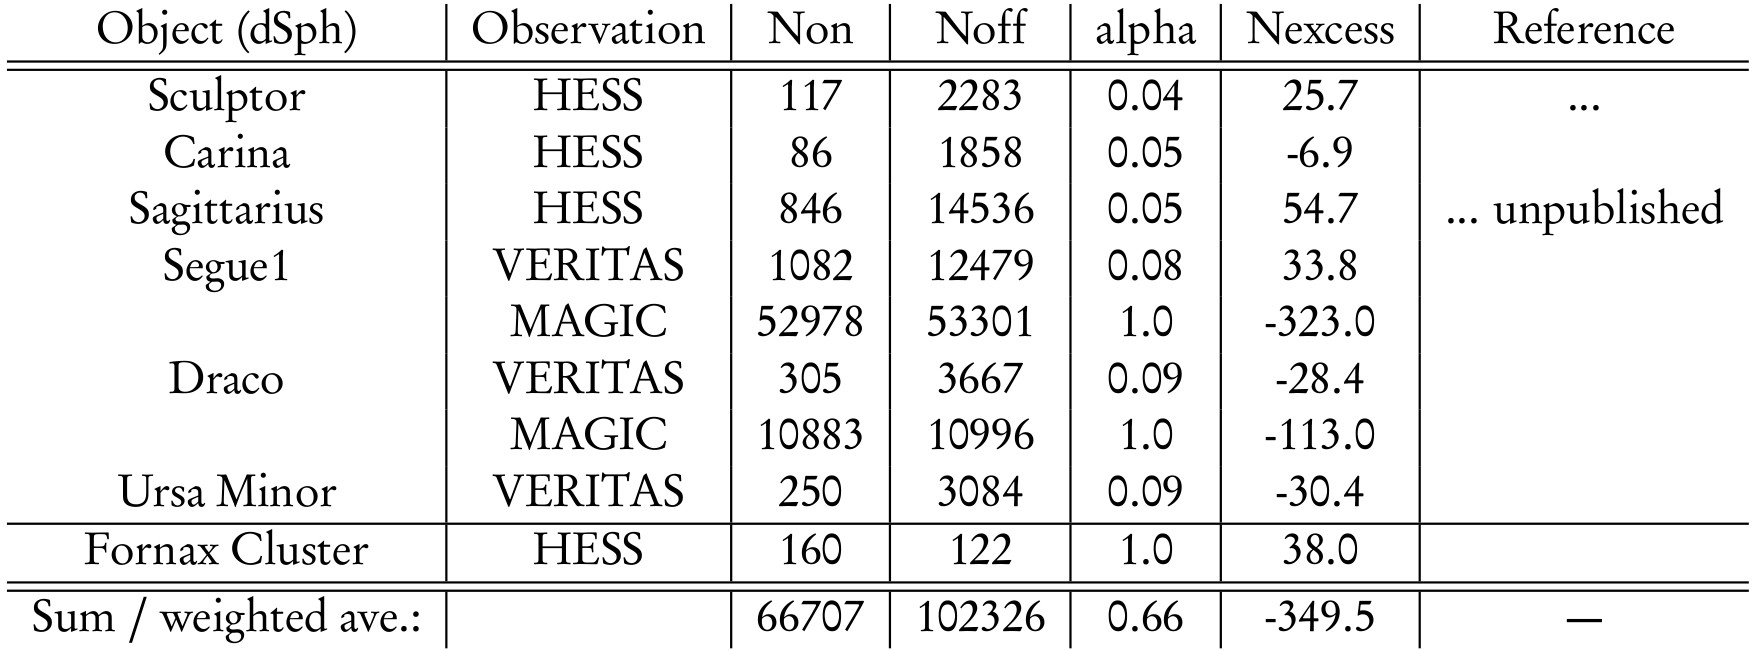
\includegraphics[width=\textwidth]{Data1_Nevents.jpg}
  \end{figure}

\end{frame}
%%%%%%%%%%%%%%%%%%%%%%%%%%%%%%%%%%%%%%%%%%%%%%%%%%%%%%%%%%%%%%


%%%%%%%%%%%%%%%%%%%%%%%%%%%%%%%%%%%%%%%%%%%%%%%%%%%%%%%%%%%%%%%%%%%%%%%%%
\begin{frame}
  \frametitle{Data: from selected publications of highest quality}

  \begin{figure}[]
    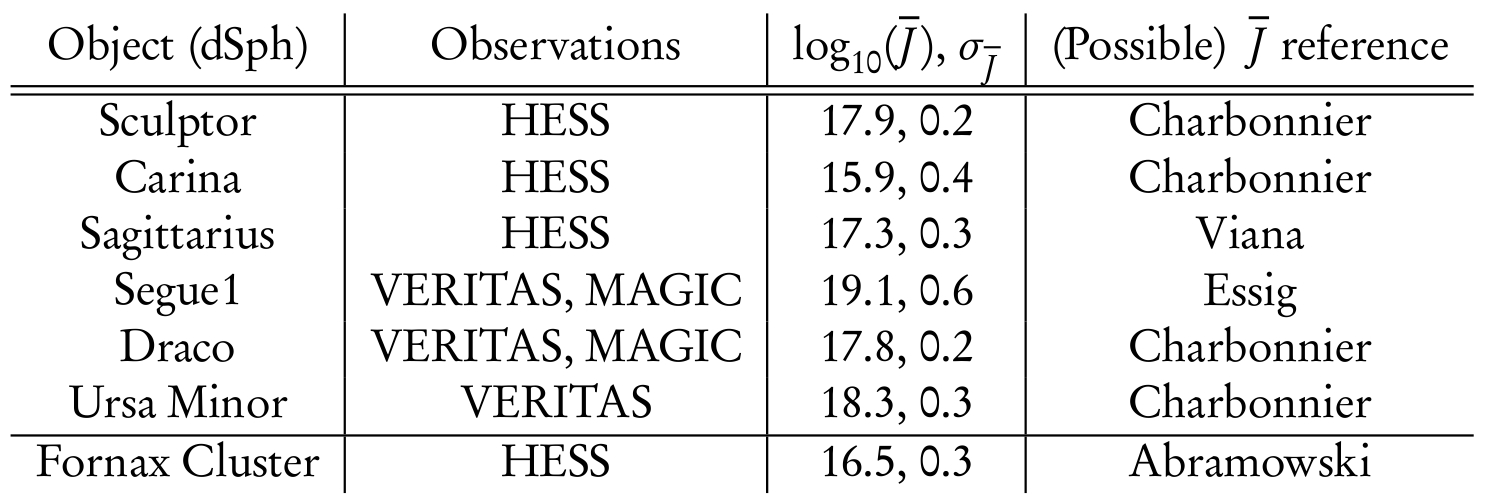
\includegraphics[width=\textwidth]{Data2_Jbars.jpg}
  \end{figure}

\end{frame}
%%%%%%%%%%%%%%%%%%%%%%%%%%%%%%%%%%%%%%%%%%%%%%%%%%%%%%%%%%%%%%

%%%%%%%%%%%%%%%%%%%%%%%%%%%%%%%%%%%%%%%%%%%%%%%%%%%%%%%%%%%%%%%%%%%%%%%%%
\begin{frame}
  \frametitle{Combined likelihood}

Hence, the full combined likelihood $\mathcal{CL}$ is a function of:
\bit
  \item  $\sigmav$, $m_\chi$ and the (``true'') \jbar factors of all
    targets \\ (these are the ``free'' parameters!)
  \item the experimental parameters of each observation ($T_{\sf obs}, A_{\sf eff}$) 
  \item the experimental results (\non, \noff)
\eit 

 ~ 

Next step: 

Calculate combined profile likelihood $\mathcal{PL}$,
as a function of fixed $\sigmav_f$, for fixed DM masses $m_f$ \ra
maximize $\mathcal{CL}$ over the $\jbar$'s:

\beq
-2 \ln \mathcal{PL}(\sigmav_f, m_f) = -2 \ln \left( \frac{\max\left[\mathcal{CL}(\sigmav_f,
    m_f, \{\jbar\})\right]}{\max \left[\mathcal{CL}(\sigmav, m_f, \{\jbar\})\right]} \right)
\eeq

\end{frame}
%%%%%%%%%%%%%%%%%%%%%%%%%%%%%%%%%%%%%%%%%%%%%%%%%%%%%%%%%%%%%%


%%%%%%%%%%%%%%%%%%%%%%%%%%%%%%%%%%%%%%%%%%%%%%%%%%%%%%%%%%%%%%%%%%%%%%%%%
\begin{frame}
  \frametitle{Profile likelihoods}

  \begin{figure}[]
    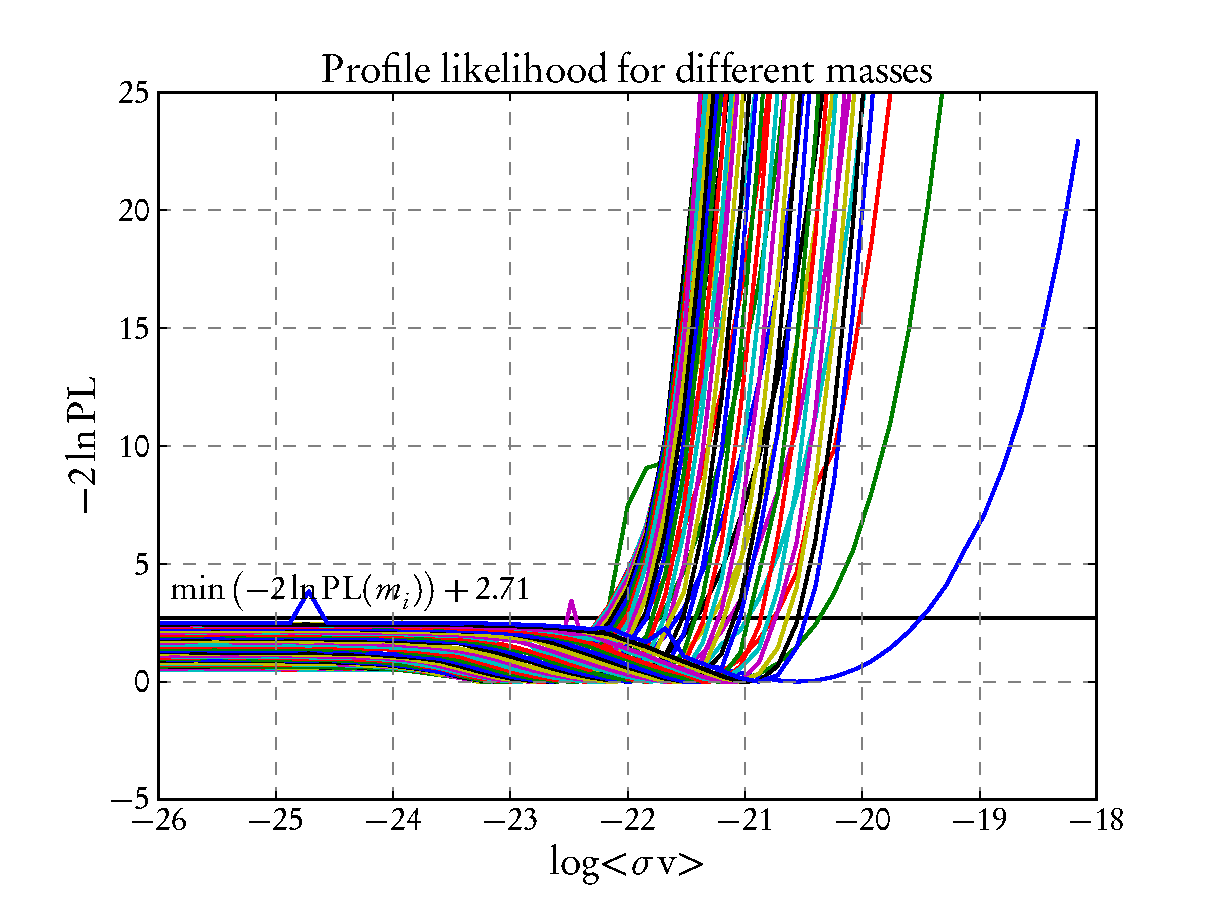
\includegraphics[width=.9\textwidth]{2012-10-05_50steps_PLs_neuerPlot.pdf}
  \end{figure}

\end{frame}
%%%%%%%%%%%%%%%%%%%%%%%%%%%%%%%%%%%%%%%%%%%%%%%%%%%%%%%%%%%%%%
%%%%%%%%%%%%%%%%%%%%%%%%%%%%%%%%%%%%%%%%%%%%%%%%%%%%%%%%%%%%%%%%%%%%%%%%%
\begin{frame}
  \frametitle{Results: Combined upper limit on \sigmav}

  \begin{figure}[]
    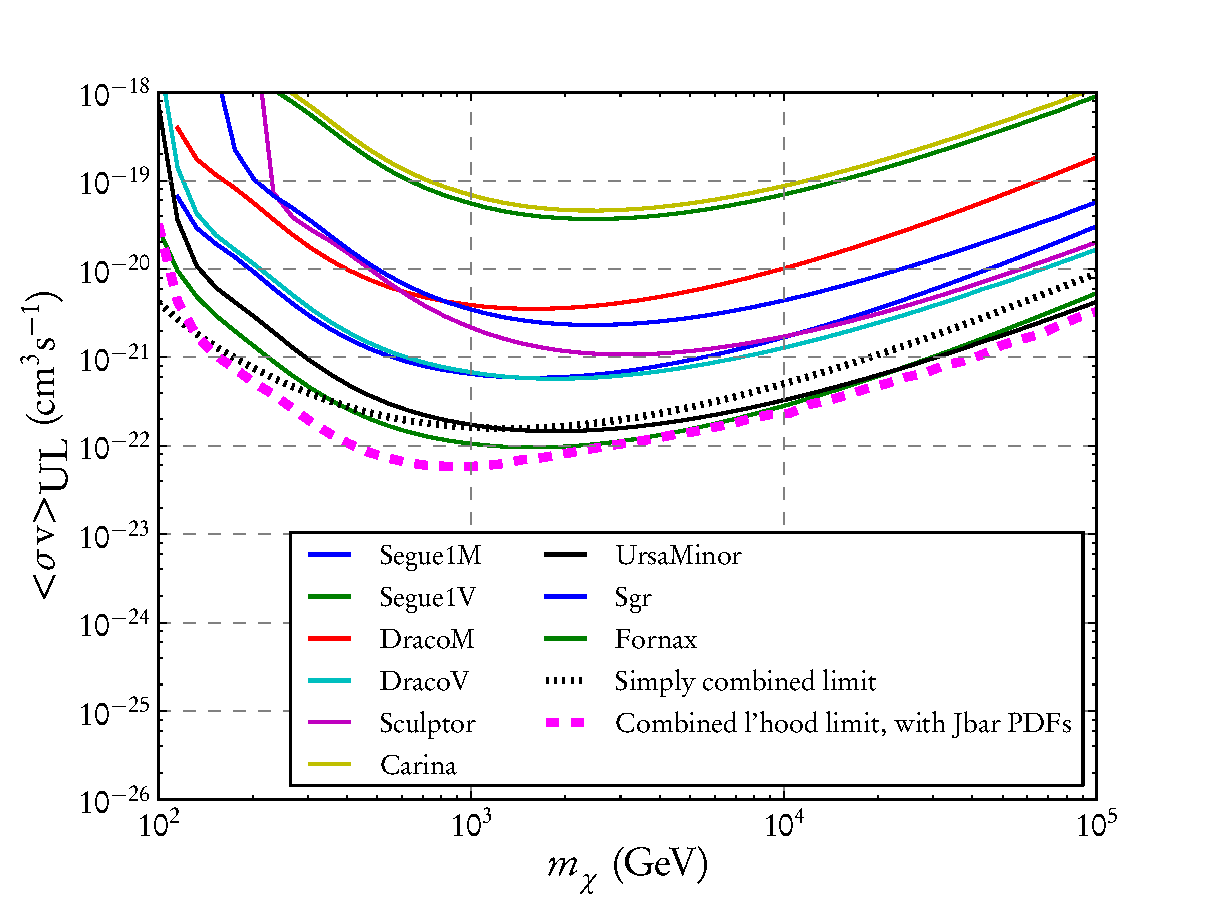
\includegraphics[width=.9\textwidth]{2012-10-05_50steps_Excl_neuerPlot.pdf}
  \end{figure}

\end{frame}
%%%%%%%%%%%%%%%%%%%%%%%%%%%%%%%%%%%%%%%%%%%%%%%%%%%%%%%%%%%%%%

%%%%%%%%%%%%%%%%%%%%%%%%%%%%%%%%%%%%%%%%%%%%%%%%%%%%%%%%%%%%%%%%%%%%%%%%%
\begin{frame}
  \frametitle{``Backup'': Results: negative excess obs. only} 
% \vspace{-1mm}
% Only observations with negative excess:
% \vspace{-3mm}
  \begin{figure}[]
    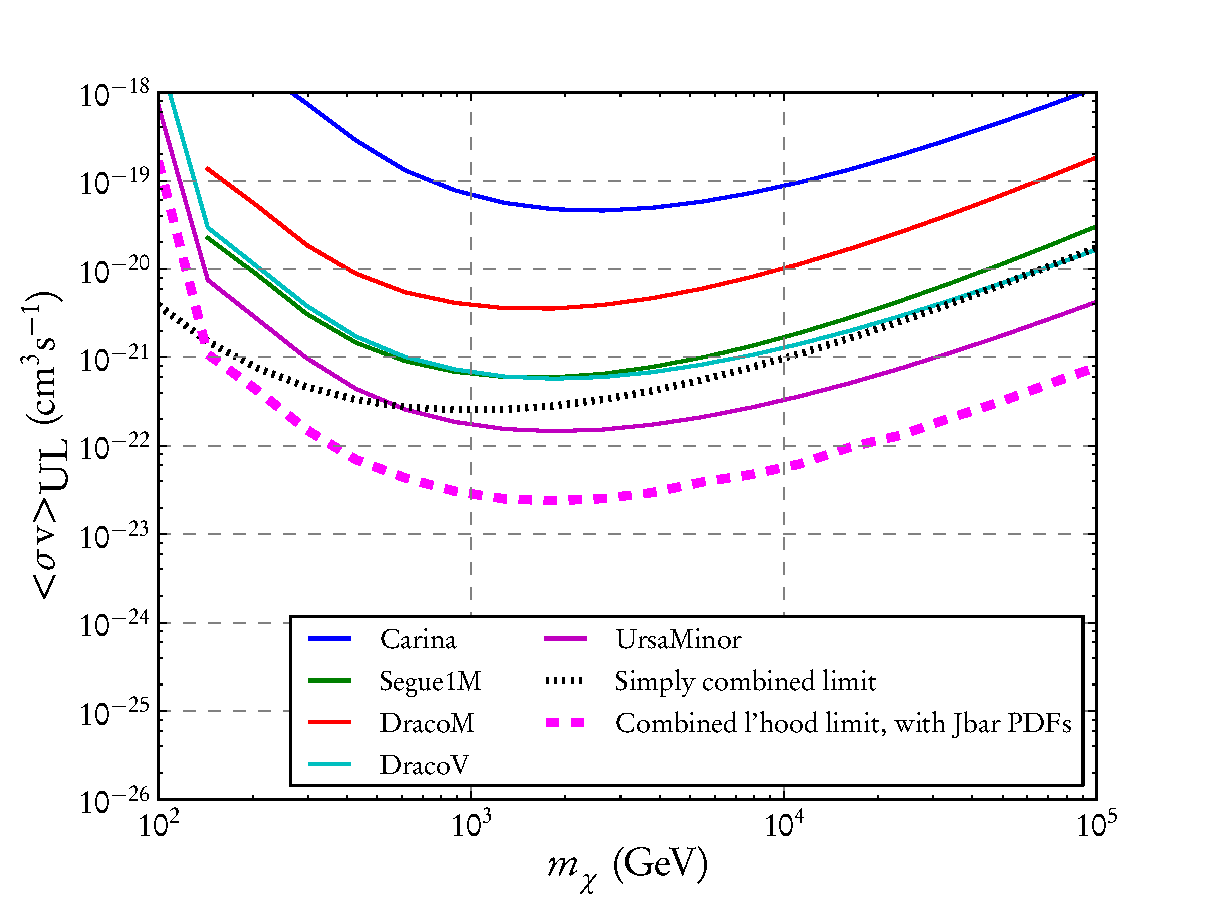
\includegraphics[width=.9\textwidth]{2012-10-05_negativeExcesses_Excl_neuerPlot.pdf}
  \end{figure}

\end{frame}
%%%%%%%%%%%%%%%%%%%%%%%%%%%%%%%%%%%%%%%%%%%%%%%%%%%%%%%%%%%%%%

%%%%%%%%%%%%%%%%%%%%%%%%%%%%%%%%%%%%%%%%%%%%%%%%%%%%%%%%%%%%%%%%%%%%%%%%%
\begin{frame}
  \frametitle{Profile likelihoods}
Only observations with negative excess:
  \begin{figure}[]
    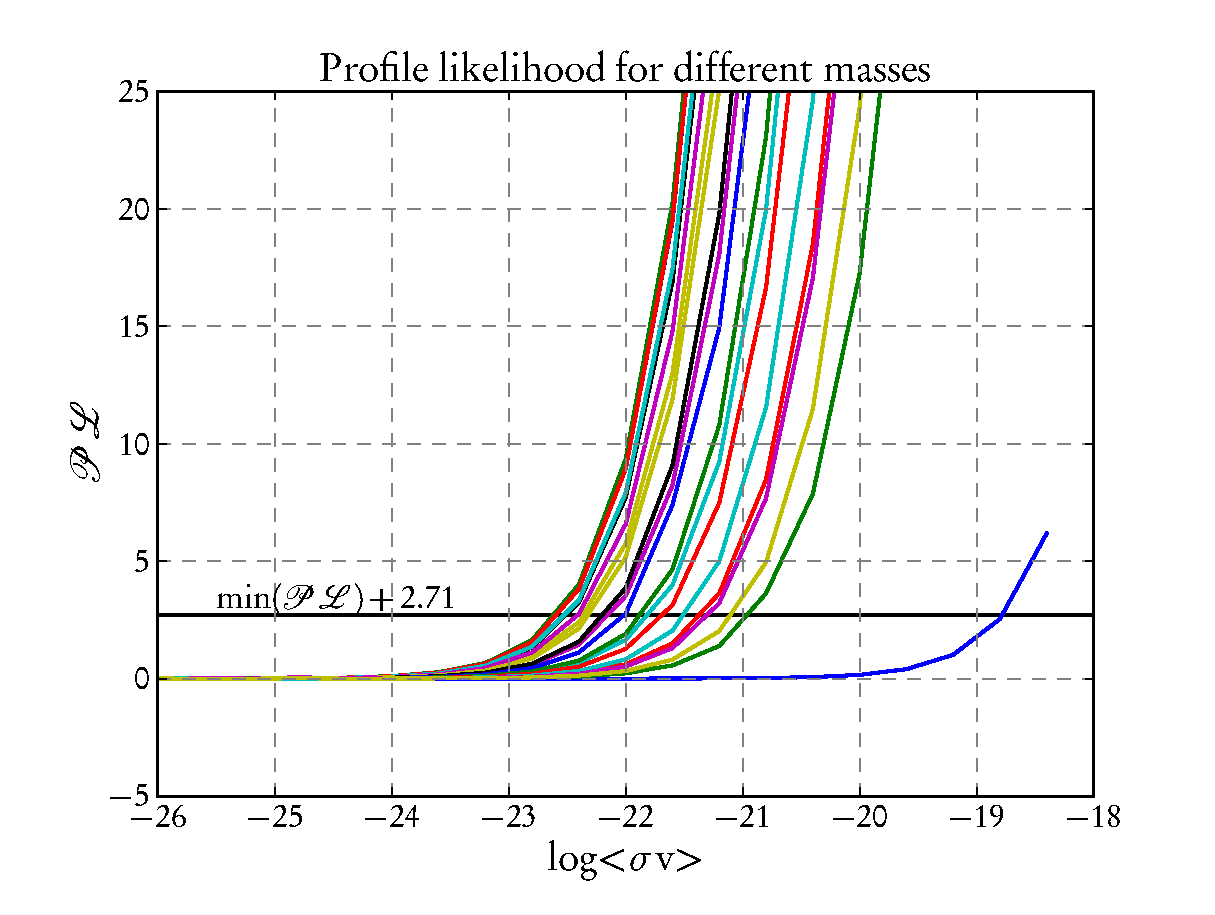
\includegraphics[width=0.8\textwidth]{2012-10-05_negativeExcesses_PLs.pdf}
  \end{figure}

\end{frame}
%%%%%%%%%%%%%%%%%%%%%%%%%%%%%%%%%%%%%%%%%%%%%%%%%%%%%%%%%%%%%%
%%%%%%%%%%%%%%%%%%%%%%%%%%%%%%%%%%%%%%%%%%%%%%%%%%%%%%%%%%%%%%%%%%%%%%%%%
\begin{frame}
  \frametitle{Profile likelihoods}
Only observations with positive excess:
  \begin{figure}[]
    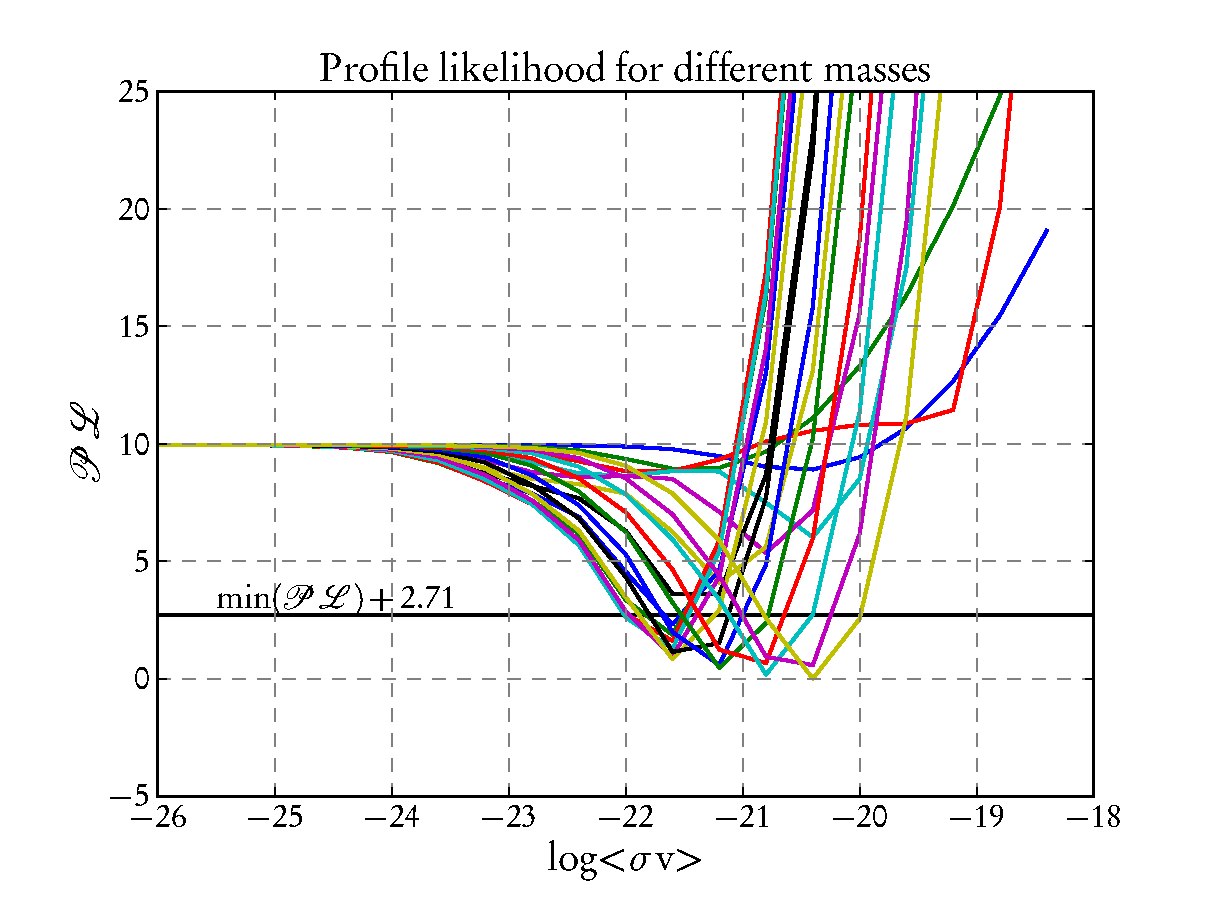
\includegraphics[width=.8\textwidth]{2012-10-05_positiveExcesses_PLs.pdf}
  \end{figure}

\end{frame}
%%%%%%%%%%%%%%%%%%%%%%%%%%%%%%%%%%%%%%%%%%%%%%%%%%%%%%%%%%%%%%

%%%%%%%%%%%%%%%%%%%%%%%%%%%%%%%%%%%%%%%%%%%%%%%%%%%%%%%%%%%%%%%%%%%%%%%%%
\begin{frame}
  \frametitle{Latest run}
  \begin{figure}[]
    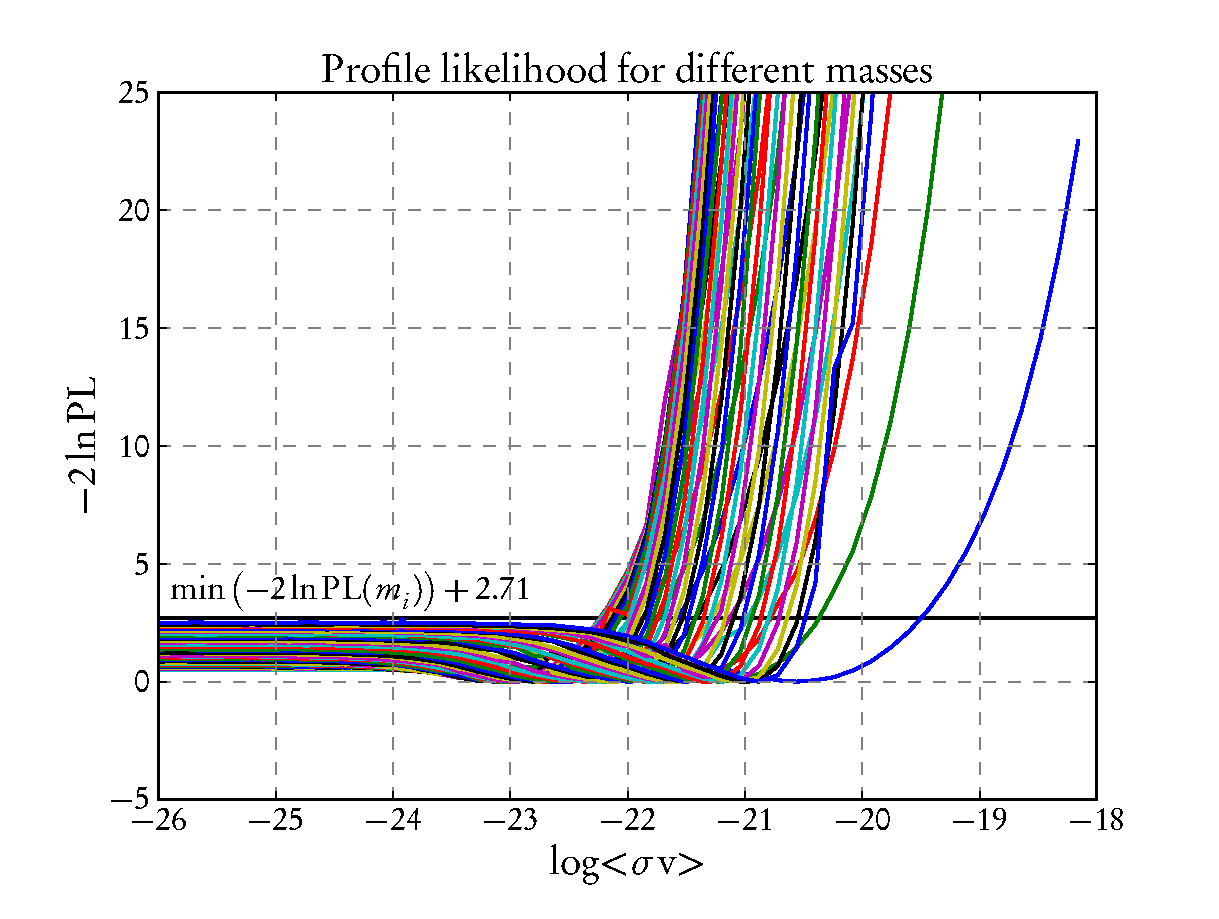
\includegraphics[width=0.8\textwidth]{2012-10-10_50steps_PLs.pdf}
  \end{figure}
\end{frame}
%%%%%%%%%%%%%%%%%%%%%%%%%%%%%%%%%%%%%%%%%%%%%%%%%%%%%%%%%%%%%%
%%%%%%%%%%%%%%%%%%%%%%%%%%%%%%%%%%%%%%%%%%%%%%%%%%%%%%%%%%%%%%%%%%%%%%%%%
\begin{frame}
  \frametitle{Latest run}
  \begin{figure}[]
    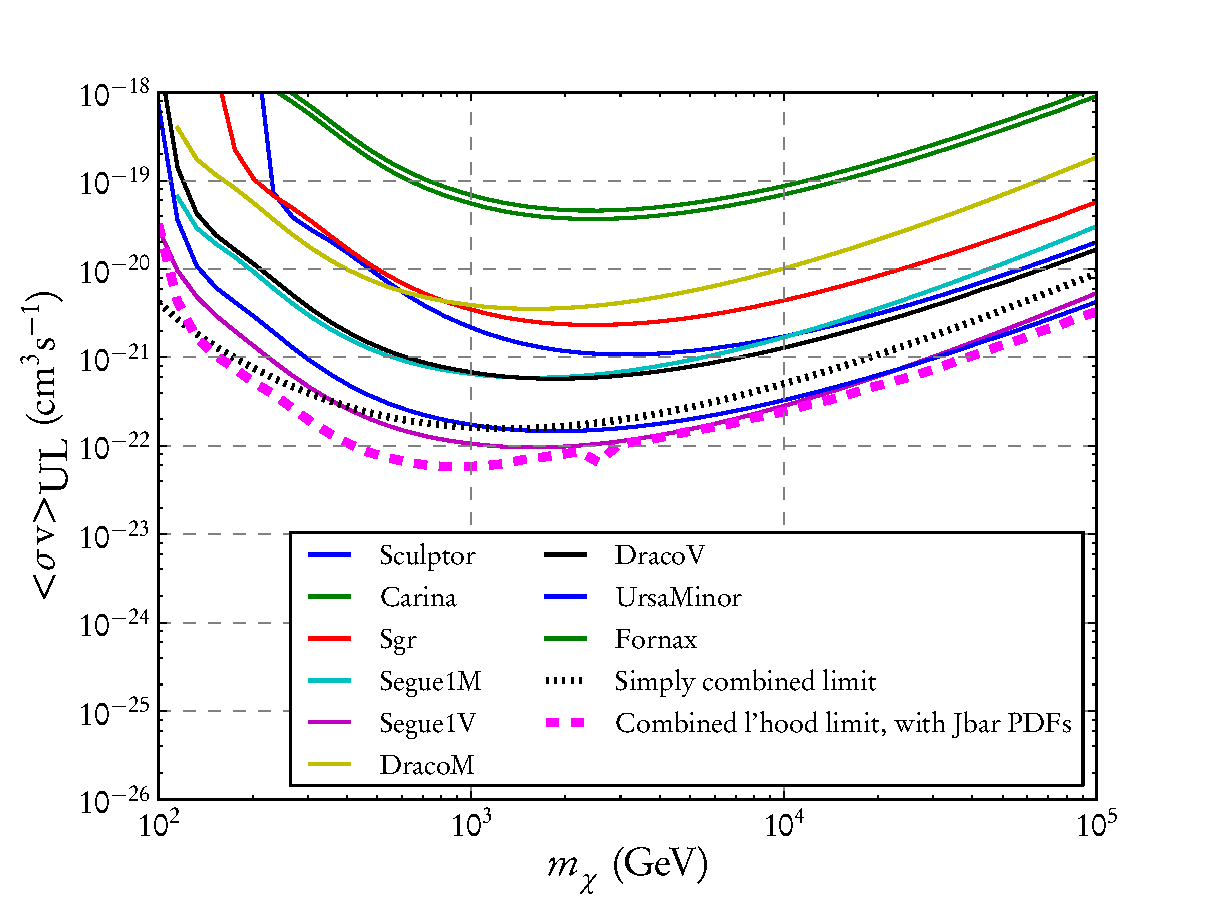
\includegraphics[width=.8\textwidth]{2012-10-10_50steps_Excl.pdf}
  \end{figure}
\end{frame}
%%%%%%%%%%%%%%%%%%%%%%%%%%%%%%%%%%%%%%%%%%%%%%%%%%%%%%%%%%%%%%

%%%%%%%%%%%%%%%%%%%%%%%%%%%%%%%%%%%%%%%%%%%%%%%%%%%%%%%%%%%%%%%%%%%%%%%%%
\begin{frame}
  \frametitle{Issues}
\bit
  \item How to deal with ``negative excesses'', or their influence on
    the resulting UL?
    \bit
      \item Implement profile likelihood for parameter $b$?
    \eit
  \item Stability of minimizations ...
  \item Implement profile likelihood for single observation limits?
  \item 
  \item 
  \item 
\eit

\end{frame}
%%%%%%%%%%%%%%%%%%%%%%%%%%%%%%%%%%%%%%%%%%%%%%%%%%%%%%%%%%%%%%

\setcounter{framenumber}{9}
\end{document}
%%%%%%%%%%%%%%%%%%%%%%%%%%%%%%%%%%%%%%%%%%%%%%%%%%%%%%%%%%%%%%
%%%%%%%%%%%%%%%%%%%%%%%%%%%%%%%%%%%%%%%%%%%%%%%%%%%%%%%%%%%%%%
%%%%%%%%%%%%%%%%%%%%%%%%%%%%%%%%%%%%%%%%%%%%%%%%%%%%%%%%%%%%%%
%%%%%%%%%%%%%%%%%%%%%%%%%%%%%%%%%%%%%%%%%%%%%%%%%%%%%%%%%%%%%%
%%%%%%%%%%%%%%%%%%%%%%%%%%%%%%%%%%%%%%%%%%%%%%%%%%%%%%%%%%%%%%
%%%%%%%%%%%%%%%%%%%%%%%%%%%%%%%%%%%%%%%%%%%%%%%%%%%%%%%%%%%%%%
%%%%%%%%%%%%%%%%%%%%%%%%%%%%%%%%%%%%%%%%%%%%%%%%%%%%%%%%%%%%%%
%%%%%%%%%%%%%%%%%%%%%%%%%%%%%%%%%%%%%%%%%%%%%%%%%%%%%%%%%%%%%%
%%%%%%%%%%%%%%%%%%%%%%%%%%%%%%%%%%%%%%%%%%%%%%%%%%%%%%%%%%%%%%
%%%%%%%%%%%%%%%%%%%%%%%%%%%%%%%%%%%%%%%%%%%%%%%%%%%%%%%%%%%%%%
%%%%%%%%%%%%%%%%%%%%%%%%%%%%%%%%%%%%%%%%%%%%%%%%%%%%%%%%%%%%%%
%%%%%%%%%%%%%%%%%%%%%%%%%%%%%%%%%%%%%%%%%%%%%%%%%%%%%%%%%%%%%%
%%%%%%%%%%%%%%%%%%%%%%%%%%%%%%%%%%%%%%%%%%%%%%%%%%%%%%%%%%%%%%



%%%%%%%%%%%%%%%%%%%%%%%%%%%%%%%%%%%%%%%%%%%%%%%%%%%%%%%%%%%%%%%%%%%%%%%%%
\begin{frame}
  \frametitle{Numerische Integration f�r Anf�nger}

 	



\begin{align*}
\int_0^{\frac{\pi}{2}} d\theta \sin \theta \exp \left( -
    \frac{\theta^2}{2 \cdot 
  (0.0175)^2} \right)  & =  3.062187\times 10^{-4} \\
\uncover<2->{\int_0^1 d(\cos\theta) \exp \left( - \frac{\arccos^2 (\cos
      \theta)}{2 \cdot   (0.0175)^2} \right)  & =  3.062187\times
  10^{-4}  \\} 
\uncover<3->{\int_0^{\frac{\pi}{2}} d\theta \sin \theta \exp \left( - \frac{\theta^2}{2 \cdot
  (0.00175)^2} \right)  & =  3.062496\times 10^{-6} \\}
\uncover<4->{\int_0^1 d(\cos\theta) \exp \left( - \frac{\arccos^2
      (\cos \theta)}{2 \cdot   (0.00175)^2} \right)  & =
  2.972690\times 10^{-157} &&  \textsf{ (Python)} \\  }
\uncover<5->{& = 0.0  && \textsf{ (Maple 11)} \\ }
\uncover<6->{& =    2.972690\times 10^{-157} && \textsf{ (Maple 12)} }
\end{align*}


% \begin{eqnarray*}
% \int_0^{\pi/2} d\theta \sin \theta \exp \left( - \frac{\theta^2}{2 \cdot
%   (0.0175)^2} \right)  &=&  3.062187\times 10^{-4}  \pause\\
% \int_0^1 d(\cos\theta) \exp \left( - \frac{\arccos^2 (\cos \theta)}{2 \cdot
%   (0.0175)^2} \right)  &=& 3.062187\times 10^{-4}  \pause\\
% \int_0^{\pi/2} d\theta \sin \theta \exp \left( - \frac{\theta^2}{2 \cdot
%   (0.00175)^2} \right)  &=&  3.062496\times 10^{-6}  \pause\\
% \int_0^1 d(\cos\theta) \exp \left( - \frac{\arccos^2 (\cos \theta)}{2 \cdot
%   (0.00175)^2} \right)  &=&  2.972690\times 10^{-157} \hfill \textsf{
% (Python)}  \pause \\ 
% &=& 0.0 \hfill \textsf{ (Maple 11)} \pause \\
% &=&    2.972690\times 10^{-157} \hfill  \textsf{ (Maple 12)} \pause
% \end{eqnarray*}


%  \begin{figure}[]
%    \includegraphics[width=\textwidth]{AsterixEnde} %
%  \end{figure}

\end{frame}
%%%%%%%%%%%%%%%%%%%%%%%%%%%%%%%%%%%%%%%%%%%%%%%%%%%%%%%%%%%%%%

%%%%%%%%%%%%%%%%%%%%%%%%%%%%%%%%%%%%%%%%%%%%%%%%%%%%%%%%%%%%%%%%%%%%%%%%%
\section[Introduction]{Introduction}
\subsection[Indirect search for dark matter]{Indirect search for dark matter} 

\begin{frame}
  \frametitle{Indirect search for dark matter}

\begin{alertblock}{\textbf{IF} dark matter particles annihilate ... or
    decay:} 
\bit
  \item final states (usually) decay hadronically \\ \ra production of
  very-high-energy (VHE) $\gamma$'s by $\pi_0$ decay
  \item or production of $\gamma \gamma$ or $\gamma Z$ lines via loop processes
\eit

\ra look for VHE $\gamma$'s coming from regions with high DM
density %\\
%\ra and for antimatter: diffuse flux of charged particles 

\end{alertblock}

\begin{block}{Photon flux calculation: self-annihilation}
\bit
  \item Differential flux:
    $\frac{d\Phi(\Delta\Omega,E_{\gamma})}{dE_{\gamma}}\,=\frac{1}{8\pi}\,
    \underbrace{\frac{\langle \sigma    v\rangle}{m^2_{\textsf{DM}}}
      \,\frac{dN_{\gamma}}{dE_{\gamma}}}_{\textsf{particle physics}}   
    \,\times\,\underbrace{\bar{J}(\Delta\Omega)
      \Delta\Omega}_{\textsf{astrophysics}} $
  \item ``halo factor'': 
    $\overline{J}(\Delta \Omega) =
    \frac{1}{\Delta\Omega}\int_{\Delta\Omega} d\Omega 
    \int_{\textsf{l.o.s.}} dl \cdot \rho^2(l)$ 

    \vspace{1mm}
    [$\Delta \Omega$(HESS) $\approx 2 \cdot 10^{-5}$ sr]
  \item decaying DM: $\overline{J} \propto \int \rho$ \ra not considered
%    $\frac{d\Phi(\Delta\Omega,E_{\gamma})}{dE_{\gamma}}\,=\frac{1}{8\pi}\,
%    \underbrace{\frac{\langle \sigma v\rangle}{m^2_{DM}}\,
%    \frac{dN_{\gamma}}{dE_{\gamma}}}_{\textsf{particle physics}}  
%    \,\times\,\underbrace{\bar{J}(\Delta\Omega)
%      \Delta\Omega}_{\textsf{Astrophysics}} $
\eit

%... but we can't see decaying DM, so I will focus on annihilation in
%the following.

\end{block}

\end{frame}



%%%%%%%%%%%%%%%%%%%%%%%%%%%%%%%%%%%%%%%%%%%%%%%%%%%%%%%%%%%%%%%%%%%%%%%%%
\subsection[Features of DM candidate particles]{Features of DM
  candidate particles}  

\begin{frame}
  \frametitle{Features of DM candidate particles}

\begin{columns}
  \column{.60\textwidth}
\begin{block}{Mostly studied: Supersymmetry ...}
\bit 
  \item continuous $\gamma$ flux from neutralino annihilation
  \item here: peak from ``virtual brems- strahlung'' [JHEP 0801,049
    (2008)] \\  --- cf. Ripken et al., ICRC '09 
    %yet considered at H.E.S.S.  
\eit
\end{block}

\begin{block}{... or extra dimensions}
\bit
  \item first KK excitation $\tilde{B}(1)$ as DM particle (here: 6 dim.) 
  \item spectrum with hard cut-off \\ {} [PRD 80,023512 (2009)] 
\eit

\end{block}
%(or both: see outlook)

  \column{.40\textwidth}
%  \vspace{5mm}
  \begin{figure}[]
    \includegraphics[width=\textwidth]{BM4.pdf}
  \end{figure}

  \begin{figure}[]
    \includegraphics[width=\textwidth]{Continuum.pdf}
  \end{figure}

\end{columns}


\end{frame}

%%%%%%%%%%%%%%%%%%%%%%%%%%%%%%%%%%%%%%%%%%%%%%%%%%%%%%%%%%%%%%%%%%%%%%%%%
\subsection[Possible sources of a DM signal]{Possible sources of a DM signal}

\begin{frame}
  \frametitle{Possible sources of a DM signal}


\begin{columns}
\column{.50\textwidth}
\begin{block}{Centre of the Milky Way}
    \bit 
      \item H.E.S.S. source J1745-290 \\ coincident with Sgr A*
	\\ {} [arXiv:0811.0931] 
%      \item H.E.S.S. TeV $\gamma$ source
    \eit
\end{block}
  \column{.50\textwidth}
\begin{figure}[]
  \includegraphics[width=0.7\textwidth]{ImprovedPosition.pdf}
  %{HESS_GC_2}
  %{Eintracht_Frankfurt_Logo.png}
  % [width=0.8\textwidth,height=0.28\textheight]{Dwarfs2} 
  % -title_image} 
\end{figure}
\end{columns}


\begin{columns}
\column{.50\textwidth}
\begin{block}{Local clumps of dark matter \\(without visible counterpart)}
    \bit 
      \item DM ``mini-spikes'' \\  {} [PRD 72,103517 (2005)] 
    \eit
\end{block}
  \column{.50\textwidth}
\begin{figure}[]
  \includegraphics[width=0.6\textwidth, height=0.3\textheight]{Aquarius}
  % -title_image} 
\end{figure}
\vspace{-5mm}
\hfill 
{\tiny \texttt{www.mpa-garching.mpg.de/aquarius}}
\end{columns}

\end{frame}


%%%%%%%%%%%%%%%%%%%%%%%%%%%%%%%%%%%%%%%%%%%%%%%%%%%%%%%%%%%%%%%%%%%%%%%%%
\begin{frame}
  \frametitle{Possible sources of a DM signal (II)}

\begin{columns}
\column{.60\textwidth}
\begin{block}{Dwarf spheroidal galaxies [0902.3492]}
    \bit 
      \item most extremely DM-dominated galaxies [ApJ 678,614 (2008)]
      \item high M/L
      \item no astrophysical $\gamma$-ray background
    \eit
\end{block}

  \column{.40\textwidth}
\hfill
\begin{figure}[]
  \includegraphics[width=0.7\textwidth]{Dwarfs_links_2}
  % -title_image} 
\end{figure}
\end{columns}

\begin{columns}
\column{.45\textwidth}
\begin{block}{(Clusters of) Galaxies}
    \bit 
%      \item large, gravitationally bound objects
      \item DM predictions: \\ {}
        [PRD 61,023514 (1999)], \\ {}
        [A\&A 455,21 (2006)] ~
        %[PRD 70,103529 (2004)], \\ ~
    \eit
\end{block}

  \column{.55\textwidth}
\begin{figure}[]
  \includegraphics[width=0.4\textwidth]{M87_jet_v2.jpg} ~
  \includegraphics[width=0.4\textwidth]{bullet-cluster-square.jpg}
\end{figure}
\end{columns}
\begin{block}{``free extra'':}
\bit 
  \item Cosmic ray electrons + positrons
\eit
\end{block}

% \begin{figure}[]
%   \includegraphics[width=0.8\textwidth,height=0.28\textheight]{Dwarfs2} 
%   % -title_image} 
% \end{figure}

% \begin{block}{Ordered by increasing distance: regions of \textbf{high}
%       DM density}
% \bit 
%   \item Centre of the Milky Way
%   \item Intermediate mass black holes / ``mini-spikes'' of DM
%   \item Dwarf Spheroidals: most extremely DM-dominated galaxies
%   \item Extragalactic sources: (clusters of) galaxies
% \eit
% \end{block}

% Bildchen: GC (HESS), M87 (Hubble), bullet cluster (?)

\end{frame}

%%%%%%%%%%%%%%%%%%%%%%%%%%%%%%%%%%%%%%%%%%%%%%%%%%%%%%%%%%%%%%%%%%%%%%%%%
\section[H.E.S.S. searches]{H.E.S.S. searches}
% \subsection[H.E.S.S. searches]{}
% %{H.E.S.S. searches}

% \begin{frame}
%   \frametitle{H.E.S.S. searches}
% ... gibt's ein Bild, das zeigt, welcher Teil des Himmels fuer HESS
%   sichtbar ist? Sonst: Plane scan


% \begin{block}{Ordered by increasing distance:}
% \bit 
%   \item Galactic centre: Sgr A*
%   \item Intermediate mass black holes: Galactic plane scan
%   \item Dwarf spheroidal galaxies: Sagittarius dSph, Canis Major (?)
%   \item Extragalactic sources: M87, Coma galaxy cluster
% \eit
% \end{block}

% \begin{alertblock}{``FREE EXTRA'':}
% \bit 
%   \item Cosmic ray electrons + positrons
% \eit
% \end{alertblock}

% \end{frame}

%%%%%%%%%%%%%%%%%%%%%%%%%%%%%%%%%%%%%%%%%%%%%%%%%%%%%%%%%%%%%%%%%%%%%%%%%
\subsection[Galactic centre]{Galactic centre}

\begin{frame}
  \frametitle{Galactic centre} 

\begin{alertblock}{d = 8 kpc, M $\approx$ 10$^6$ M$_\Sun$ }
\begin{itemize}
  \item\textbf{Bonus:} Nearby source of TeV photons
  \item\textbf{Malus:} Spectrum doesn't look like dark matter
\end{itemize}
\end{alertblock}


\begin{columns}
  \column{.40\textwidth}
  \vspace{-5mm}
  \begin{figure}[]
    \includegraphics[width=\textwidth,height=0.45\textheight]{11569fg2a.pdf}
    %SpectresDM.pdf}
  \end{figure}

  \column{.60\textwidth}

\begin{block}{PRL 97,221102 (2006)}
\bit
  \item strong source coincident with Sgr A*
  \item spectrum well-fit by a power law \\with cut-off above 10 TeV \\ {}
    [A\&A 503,817 (2009)]
  \item un-identified astrophysical source produces \emph{bulk} of emission
\eit
\end{block}

\end{columns}

\begin{block}{}
  Fit of power-law background + DM signal models to spectrum \\ \ra robust
  calculation of upper limits: $\langle \sigma v\rangle \leq 1 \cdot
    10^{-24}$ cm$^3$/s
\end{block}


\end{frame}



%%%%%%%%%%%%%%%%%%%%%%%%%%%%%%%%%%%%%%%%%%%%%%%%%%%%%%%%%%%%%%%%%%%%%%%%%
\subsection[Sagittarius Dwarf Spheroidal galaxy]{Dwarf Spheroidals}
%{Sagittarius Dwarf Spheroidal galaxy} 

\begin{frame}
  \frametitle{Sagittarius Dwarf Spheroidal galaxy}

\begin{alertblock}{d = 25 kpc, M $\approx$ 10$^6$ M$_\Sun$ } %$_{\textsf{PSF}}$
\begin{itemize}
  \item\textbf{Bonus:} Close, large dwarf spheroidal
  \item\textbf{Malus:} No signal. Upper limit on integrated flux
    (E$_\gamma$ > 250 GeV) 
\end{itemize}
\end{alertblock}

\begin{columns}
  \column{.40\textwidth}
\vspace{-4mm}
  \begin{figure}[]
    \includegraphics[width=0.9\textwidth,height=0.3\textheight]{Moulin_Sgr_Neu2}
  \end{figure}
\vspace{-7mm}
  \begin{figure}[]
    \includegraphics[width=0.9\textwidth,height=0.3\textheight]{KK.jpg}
  \end{figure}


  \column{.60\textwidth}

\begin{block}{Astrop. Phys. 29,55 (2008)}
\bit
  \item 11 h of data
  \item $\Phi_{\textsf{Int}} \leq 3.6 \cdot 10^{-12}$ /cm$^2$s 
  \item Two diff. profile models (NFW): $\overline{J} = 2.2 \cdot 10^{24}$
    GeV$^2$/cm$^{5}$ (``cusped''),  $\overline{J} = 75 \cdot 10^{24}$
    GeV$^2$/cm$^{5}$ (``cored'') 
  \item SUSY limit: $\langle \sigma v\rangle \leq 5 \cdot
    10^{-24}$ cm$^3$/s
  \item KK limit: $\langle \sigma v\rangle \leq 1 \cdot 10^{-24}$ cm$^3$/s
  \item both for cusped NFW profile, \\ at 95\% C.L., for m$_\chi \sim$ 1 TeV
\eit
\end{block}

\end{columns}


\end{frame}


%%%%%%%%%%%%%%%%%%%%%%%%%%%%%%%%%%%%%%%%%%%%%%%%%%%%%%%%%%%%%%%%%%%%%%%%%
\subsection[Canis major overdensity]{}%{Canis major overdensity}

\begin{frame}
  \frametitle{Canis major overdensity}

\begin{alertblock}{d = 8 kpc, M = ?}
\begin{itemize}
  \item\textbf{Bonus:} Very close! Good candidate for DM signal.
  \item\textbf{Malus:} Status as a Dwarf Spheroidal under
    dispute. Properties not well constrained; tidally disrupted
\end{itemize}
\end{alertblock}

\begin{columns}
  \column{.45\textwidth}
  % \vspace{-40mm}
  \begin{figure}[]
    \includegraphics[width=\textwidth]{f4a.pdf}
  \end{figure}
\vspace{-5mm}  
\bit
  \item black (red) points: MSSM models (WMAP OK)
\eit 
  \column{.60\textwidth}

\begin{block}{ApJ 691,175 (2009)}
\bit
  \item 9.6 h of data
  \item Assumptions: M$_{\textsf{halo}} \approx 3 \cdot 10^8$
    M$_{{\tiny\astrosun}}$, \\
    NFW DM profile
  \item \ra $\overline{J} = 5.9 \cdot 10^{24}$ GeV$^2$/cm$^{5}$
  \item SUSY limit: $\langle \sigma v\rangle \leq %5 \cdot
    10^{-23}$ cm$^3$/s
  \item KK limit: $\langle \sigma v\rangle \leq %5 \cdot
    10^{-24}$ cm$^3$/s
  \item both at 95\% C.L., for m$_\chi \sim$ 1 TeV
\eit
\end{block}

\end{columns}

\end{frame}


%%%%%%%%%%%%%%%%%%%%%%%%%%%%%%%%%%%%%%%%%%%%%%%%%%%%%%%%%%%%%%%%%%%%%%%%%
\subsection[Intermediate mass black holes]{Intermediate mass black holes}

\begin{frame}
  \frametitle{Intermediate mass black holes}

\begin{alertblock}{d = ?, 10 < M < 10$^6$ M$_\Sun$}
\begin{itemize}
  \item\textbf{Bonus:} Should exist! 100--1000 per galaxy? DM
    ``mini-spikes'' 
  \item\textbf{Malus:} No unambiguous observation of IMBHs to date
\end{itemize}
\end{alertblock}

\begin{columns}
  \column{.45\textwidth}
  % \vspace{-40mm}
  \begin{figure}[]
    \includegraphics[width=\textwidth]{fig6.pdf}
  \end{figure}

  \column{.55\textwidth}

\begin{block}{PRD 78,072008 (2008)}
\bit
  \item IMBH: from Pop-III stars or primordial halos
  \item use Galactic plane scan, excluding known sources
  \item assume  $\sim$ 100 IMBH in Milky Way halo
%    \ra upper limits excluding some DM models
  \item SUSY limit: $\langle \sigma v\rangle \leq
    10^{-\textcolor{red}{27}}$ cm$^3$/s \\ 
    for m$_\chi > $ 1 TeV (90 \% C.L.)
\eit
\end{block}

\end{columns}

\end{frame}


%%%%%%%%%%%%%%%%%%%%%%%%%%%%%%%%%%%%%%%%%%%%%%%%%%%%%%%%%%%%%%%%%%%%%%%%%
\subsection[Radio galaxy M87]{Extragalactic sources}
%{Radio galaxy M87}

\begin{frame}
  \frametitle{Radio galaxy M87 --- centre of Virgo cluster}

\begin{alertblock}{d = 16 Mpc, M$_{\textsf{BH}}$ = 10$^9$ M$_\Sun$}
\begin{itemize}
  \item\textbf{Bonus:} Extragalactic TeV $\gamma$ source
  \item\textbf{Malus:} Temporal variation, signal too strong for DM
\end{itemize}
\end{alertblock}

\begin{columns}
  \column{.40\textwidth}
  % \vspace{-40mm}
  \begin{figure}[]
    \includegraphics[width=0.8\textwidth]{M87_MWL_1.jpg}
  \end{figure}

  \column{.60\textwidth}

\begin{block}{Science 314,1424 (2006) \\ ... and 24,444 (2009)}
\bit
  \item strong flares \ra not DM
  \item $\gamma$ flux in low state: still above DM estimations
  \item MWL campaign: VHE $\gamma$'s from core \\
    (not resolvable with ACTs) \\
%  \item not DM either: PKS 2155-304 \\ {} [arXiv:0906.2002]
\eit
\end{block}

\end{columns}

\end{frame}


%%%%%%%%%%%%%%%%%%%%%%%%%%%%%%%%%%%%%%%%%%%%%%%%%%%%%%%%%%%%%%%%%%%%%%%%%
\subsection[Coma cluster]{}%{Coma cluster}

\begin{frame}
  \frametitle{Coma cluster}

\begin{alertblock}{z = 0.023, M $\approx$ 10$^{15}$ M$_\Sun$}
\begin{itemize}
  \item\textbf{Bonus:} Giant, heavy object
  \item\textbf{Malus:} No signal
\end{itemize}
\end{alertblock}

\begin{columns}
  \column{.50\textwidth}
  % \vspace{-40mm}
  \begin{figure}[]
    \includegraphics[width=\textwidth]{12086f1a.pdf}
  \end{figure}

  \column{.50\textwidth}

\begin{block}{A\&A 502, 437--443 (2009)}
\bit
  \item 8 h of data
  \item no significant flux detection
  \item UL (99\% CL, E$_\gamma$ > 1 TeV): \\ ~
    $\Phi \leq$ 6 $\cdot$ 10$^{-13}$/cm$^2$s \\ 
    (factor $\sim$ 100 above expected dark matter signal)
  \item constraints on non-DM models derived
\eit
\end{block}

\end{columns}

\end{frame}


%%%%%%%%%%%%%%%%%%%%%%%%%%%%%%%%%%%%%%%%%%%%%%%%%%%%%%%%%%%%%%%%%%%%%%%%%
\subsection[Dwarfs vs. clusters]{}%{Coma cluster}

\begin{frame}
  \frametitle{A few more words on dwarfs and clusters}

\begin{block}{Boosts from substructures?}
\bit 
  \item Springel et al. [Nature 456,73 (2008)] predict a boost factor
    of \mbox{$\sim$ 230} from  DM substructures of a Milky Way-like
    galaxy (when looking at it from outside!)
  \item Pinzke et al. [PRD 103,181302 (2009)] note that 
    \[  
    \frac{\Phi(\textsf{Virgo Cluster})}{\Phi(\textsf{Draco dSph})} 
    \approx \left( \frac{d_{\textsf{Draco}}}{d_{\textsf{Virgo}}}\right)^2 
    \left( \frac{M_{\textsf{Virgo}}}{M_{\textsf{Draco}}}\right)^{0.83}
    \approx 3.4     
    \]
    (however, they use an unusually (?) low value of $M_{\textsf{vir}} =
    10^{\textcolor{red}{8}} M_\Sun$ for Draco's virial mass)
  \item Unlike galaxy clusters, dwarf spheroidals  have (probably) lost
    their substructure by tidal stripping.
  \item So, should we look more carefully for DM annihilation signals
    from galaxy clusters? \\
    (Answer by J.-F. Glicenstein: \emph{Non.})
\eit
\end{block}


\end{frame}

%%%%%%%%%%%%%%%%%%%%%%%%%%%%%%%%%%%%%%%%%%%%%%%%%%%%%%%%%%%%%%%%%%%%%%%%%
\section{Summary \& outlook}
\subsection[Summary]{}
%Summary of H.E.S.S. searches]{Summary of H.E.S.S. searches}

\begin{frame}
  \frametitle{Summary of H.E.S.S. DM searches}

\begin{block}{No, we haven't seen it yet ...}
\bit 
  \item Searches for dark matter on different mass \&
    distance scales
  \item H.E.S.S. results \ra (among the) most constraining DM limits
  from Cherenkov telescopes 
  \item Limits on $\langle \sigma v \rangle$ vs. $m_\chi$ not reaching
    standard ``thermal WIMP'' / mSUGRA values (without substructure boosts)
    %($m_\chi \sim$ 100 GeV, $\langle \sigma v\rangle  \sim 10^{-26}$
    %cm$^3$/s) 
  \item Cross-section limits %on $\langle \sigma v\rangle$ 
    dependent on DM halo uncertainties
\eit

\end{block}

\begin{alertblock}{}
\begin{tabular}{c||c|c|c|c|c|}
  \textbf{H.E.S.S. obs.} & \textbf{GC} & \textbf{Sgr dSph} &
  \textbf{CMa} & \textbf{IMBH} & \textbf{M87}\\
\hline
\hline
t$_{\textsf{obs}}$ (h) & 64 & 11 & 10 & ($\sim$ 400) & 89 \\
\hline
d (kpc) & 8 & 25 & 8 & (?) & 16000 \\
\hline
Core mass (M$_\Sun$) & 10$^6$ & 10$^6$ & 10$^6$ (?) & (10$^5$ ?) & >10$^{12}$\\  
\hline
UL: $\langle \sigma v\rangle$ (cm$^3$/s) & 10$^{-24}$ & 5 $\cdot$
10$^{-24}$  & 10$^{-23}$ & 10$^{-27}$ & 10$^{-22}$ \\
\end{tabular}
\end{alertblock}

\end{frame}


%%%%%%%%%%%%%%%%%%%%%%%%%%%%%%%%%%%%%%%%%%%%%%%%%%%%%%%%%%%%%%%%%%%%%%%%%
\subsection[Outlook]{}
%[Outlook]{Outlook}

\begin{frame}
  \frametitle{Outlook}

\begin{columns}
  \column{.70\textwidth}

\begin{alertblock}{H.E.S.S. phase II --- construction ongoing ...}
\bit
  \item 5th telescope: $\diameter$ 28m  
  \item  higher sensitivity, E$_{\textsf{thresh}} \sim 30$ GeV \\
    \ra better coverage of WIMPy mass range \\
    \ra overlap with Fermi
\eit
\end{alertblock}

  \column{.30\textwidth}
  \begin{figure}[]
    \includegraphics[width=\textwidth]{PhaseII}
  \end{figure}
\end{columns}

% \begin{columns}
% \column{.35\textwidth}
%   \begin{figure}[]
%     \includegraphics[width=\textwidth]{AMSB}
%   \end{figure}

%   \column{.65\textwidth}

%\begin{block}{CTA}
%\end{block}

\begin{block}{LHC et al.}
\bit
  \item CMS has collected >15,000 collision events at 2.36 TeV!
    Unfortunately, no DM yet. :-)
  \item But: Will [\emph{enter your favourite new physics here}] be
    \textbf{the} dark matter as seen in the Universe?
%  \item \textbf{\textcolor{green!55!olive}{biodiversity}} of
  \item \textbf{\textcolor{green}{biodiversity}} of
    collider-based, direct and indirect searches: CDMS II has found
    two candidate events [0912.3592], Fermi is up and running, AMS will be
    launched on July 29 $\ldots$
  \item more to come: \textbf{CTA} 
\eit

\end{block}


% Towards using spectral information
% \bit 
%   \item H.E.S.S. limits so far: assuming power- law-like, feature-poor
%     annih. spectra
%   \item as mentioned: ``bump'' from IB
%   \item here: ``AMSB'' models with strong lines \\ {}
%     [NPB 570,455 (2000)]
% \eit

\end{frame}




%%%%%%%%%%%%%%%%%%%%%%%%%%%%%%%%%%%%%%%%%%%%%%%%%%%%%%%%%%%%%%%%%%%%%%%%%
\begin{frame}
  \frametitle{\Huge $\mathcal{THE \: END}$}
  \begin{figure}[]
    \includegraphics[width=\textwidth]{AsterixEnde} %
  \end{figure}

\end{frame}

%%%%%%%%%%%%%%%%%%%%%%%%%%%%%%%%%%%%%%%%%%%%%%%%%%%%%%%%%%%%%%%%%%%%%%%%%

\section*{}

%%%%%%%%%%%%%%%%%%%%%%%%%%%%%%%%%%%%%%%%%%%%%%%%%%%%%%%%%%%%%%%%%%%%%%%%%
%\subsection{}
%[Outlook (II)]{Outlook (II)}

\begin{frame}
  \frametitle{Backup: Outlook (II)}

\begin{columns}
  \column{.50\textwidth}
%  {\hfill \tiny [JHEP 03,045 (2003)]}
%   \begin{figure}[]
%     \includegraphics[angle=90,width=0.8\textwidth,height=0.35\textheight]{onelep} 
%   \end{figure}
  \begin{figure}[]
    \includegraphics[width=0.8\textwidth]{AMSB}
  \end{figure}

\column{.50\textwidth}
  \begin{figure}[]
    \includegraphics[width=0.8\textwidth]{SpectrLimit_09-20_SgrNFW.pdf}
  \end{figure}

\end{columns}

\begin{alertblock}{Pre-preliminary: Analysis using spectral information}
\bit
  \item using differential (d$\Phi$/dE) flux limits from Sgr dSph ...
  \item assuming $\overline{J} = 2.2 \cdot 10^{24}$ GeV$^2$/cm$^{5}$ ...
  \item for AMSB Wino models [Nucl. Phys. B 570,455 (2000)] ...
%    \ra very high $\langle \sigma v \rangle$ ...
  \item ... part of the LHC-relevant parameter space \textbf{might} actually be
    excluded by H.E.S.S. measurements.
\eit
\end{alertblock}

\end{frame}


%\subsection[CR electrons (+ positrons)]{}%{Electrons (+ positrons)}
\begin{frame}
  \frametitle{Backup: Cosmic ray electrons (+ positrons)}

\begin{alertblock}{d < 1 kpc, m$_e$ = 4.6 $\cdot$ 10$^{-61}$ M$_\Sun$}
\begin{itemize}%{description}
  \item Bonus: Coming from everywhere! $e^+$ (cut-off) as DM signal
    %of DM annihilation.
  \item Malus: Coming from everywhere. No source backtracking.
    %Backtracking of a defined source (nearly) impossible.
\end{itemize} %{description}
\end{alertblock}


\begin{columns}
  \column{.4\textwidth}
  % \vspace{-40mm}
  \begin{figure}[]
    \includegraphics[width=\textwidth]{fig2_EL2.pdf}
  \end{figure}

  \column{.60\textwidth}

\begin{block}{PRL 101,261104 (2008) \\ and arXiv:0905.0105}
\bit
  \item elm. showers from extragal. regions with small
    $\gamma$ flux  ($\sim$5 \% expected)
  \item large coll. area \ra high statistics
  \item hadronic background rejection: ``electron likeness'' parameter from
    simulations \& Random Forest %algorithm
  \item power law break at $\sim$1 TeV, \\ ATIC peak not seen, \\ good
    agreement with Fermi 
\eit
\end{block}

\end{columns}


\end{frame}

\begin{frame}
  \frametitle{Backup: $e^\pm$ analysis -- hadronic bkgr rejection}

  \begin{figure}[]
    \includegraphics[width=0.7\textwidth]{fig1_EL_bkgr.pdf}
  \end{figure}

\end{frame}

\begin{frame}
  \frametitle{Backup: $e^\pm$ analysis -- KK peak with H.E.S.S.}

  \begin{figure}[]
    \includegraphics[width=0.7\textwidth]{fig3_EL.pdf}
  \end{figure}

\end{frame}

%\begin{frame}
%  \frametitle{Backup: electron spectrum, recalibrated}
%\begin{alertblock}{}
%Using Fermi Crab $\gamma$ spectrum  to recalibrate H.E.S.S. energy:
%\end{alertblock}
%  \begin{figure}[]
%    \includegraphics[width=0.6\textwidth]{fig1_EL_bkgr.pdf}
%  \end{figure}
%\end{frame}

\begin{frame}
  \frametitle{Backup: Effects of internal bremsstrahlung}

\begin{alertblock}{}
J. Ripken, ICRC 2009: Models excluded by GC observations 
\end{alertblock}

  \begin{figure}[]
    \includegraphics[width=\textwidth]{Joachim_1.jpg}
  \end{figure}

\end{frame}

\begin{frame}
  \frametitle{Backup: AMSB and the LHC}
\vspace{-5mm}
\begin{columns}
  \column{.50\textwidth}
  % \vspace{-40mm}
  \begin{figure}[]
    \includegraphics[angle=90,width=0.8\textwidth]{onelep.pdf}
  \end{figure}

\begin{itemize}
  \item Blue diamonds: LHC reach for AMSB models (A. Barr et al.,
    [JHEP 03,045 (2003)]) 
%  \item (see also [PLB 488,367 (2000)])
%  \item more recent considerations: [0902.4880], [0906.0957] (SUSY fits)
\end{itemize}

  \column{.50\textwidth}
  % \vspace{-40mm}
  \begin{figure}[]
    \reflectbox{
      \includegraphics[angle=90,width=0.8\textwidth]{AMSB_flat_m0_m32.pdf}
    }
  \end{figure}
 \begin{itemize}
   \item S. AbdusSalam et al.: \\ Fit to low E observables \newline 
     [PRD 80,035017 (2009)] 
%   \item NOTE: inverted axes
%   \item see also [arXiv:0906.4765], [JHEP 04,088 (2009)] 
%     % considerations: [0902.4880], [0906.0957] (SUSY fits)
 \end{itemize}
\end{columns}
\end{frame}


%\subsection*{}
% \begin{frame}
%   \frametitle{Backup: Lorentz invariance violation}

% \begin{alertblock}{d = (PKS), m = 0 }
% \begin{itemize}
%   \item\textbf{Bonus:} Interesting physics!
%   \item\textbf{Malus:} Not DM.
% \end{itemize}
% \end{alertblock}

% \end{frame}







\end{document}
%%%%%%%%%%%%%%%%%%%%%%%%%%%%%%%%%%%%%%%%%%%%%%%%%%%%%%%%%%%%%%





% \subsection[10]{Dark Matter}
% \begin{frame}
%   \frametitle{Dark Matter}
%   drei bunte bildchen \\
% \begin{block}{}
%  \begin{itemize}
%   \item lots of evidence for Dark Matter
%   \item WMAP (5yr): $\Omega_{DM}=0.1...\pm...$
%  \end{itemize}
% \end{block}

% \end{frame}

% \subsection[12]{Supersymmetry}
% \begin{frame}
%   \frametitle{SUSY and the DM density}
  
% \begin{alertblock}{Supersymmetry}
%   Alertblock! 
% \end{alertblock}

% \begin{block}{The ``Wimp miracle''}
% Thermal production and freeze-out after the Big Bang: \\
% A Wimp of mass $\sim$ 100 GeV with velocity-weighted cross-section
% $<\sigma v> \approx 3\cdot 10^{-26} cm^3/s$ gives (after propagation
% through the history of the universe) just the right value for $\Omega_{DM}$.
% \end{block}

% \end{frame}



%%%%%%%%%%%%%%%%%%%%%%%%%%%%%%%%%%%%%%%%%%%%%%%%%%%%%%%%%%%%%%%%
\section[AMSB \& dSphs]{AMSB \& dwarf spheroidals}

\subsection[AMSB]{Anomaly-mediated SUSY breaking}
\begin{frame}
  \frametitle{Anomaly-mediated SUSY breaking}

\begin{block}{WMAP Dark Matter + ``thermal wimp miracle''}
   $(m_\chi \approx $ 100 GeV)+($ \langle\sigma_{\chi\chi} v\rangle \approx
   3\cdot 10^{-\textcolor{red}{26}} $ cm$^3$/s) $\ra
   \Omega_{\textsf{DM}}h^2 = 0.11$     
\end{block}

\begin{alertblock}{AMSB: Non-thermal winos}
L. Randall et al.: SUSY broken on different ``brane'', mediated by
gravity. [NPB 570,455 (2000) + ref. therein]

\bit 
  \item Physical parameters:  M$_{3/2}, \tan \beta,
    \operatorname{sgn}(\mu)$  
  \item \emph{ad hoc} rescue parameter: univ. scalar mass m$_0$
  \item  Gaugino masses: $M_i = \frac{\beta_{g_i}}{g_i} \textsf{M}_{3/2}$ \\
    \ra $M_1:M_2:M_3 \approx 2.8:1:10 $ \\
    \ra lightest neutralino is mostly (>99\%) \textbf{wino}
%  \item  $i = 1,2,3:$ U(1), SU(2), SU(3) 
  \item Large $\sigma_{\chi\chi}$: DM density from thermal
    production too small \\ \ra enhancement from gravitino decay (or
    moduli, mult. DM, ..)
\eit
%Neutralino = Wino!
\end{alertblock}

\end{frame}

%%%%%%%%%%%%%%%%%%%%%%%%%%%%%%%%%%%%%%%%%%%%%%%%%%%%%%%%%%%%%%%%
\subsection[AMSB and the LHC]{AMSB and the LHC}

%   \column{.40\textwidth}
% \vspace{-60mm}
% \begin{figure}[]
%   \includegraphics[width=1.2\textwidth]{flux}
% \end{figure}

% \begin{itemize}
%   \item $m_\chi = 180$ GeV non-thermal relic Wino as one of the
%     $10^{500}$ explanations of     the Pamela/Fermi positrons (G. Kane
%     et al., [arXiv:0812.4555], [0906.4765]) 
% \end{itemize}

\begin{frame}
  \frametitle{AMSB and the LHC}
\vspace{-5mm}
\begin{columns}
  \column{.50\textwidth}
  % \vspace{-40mm}
  \begin{figure}[]
    \includegraphics[angle=90,width=0.8\textwidth]{onelep.pdf}
  \end{figure}

\begin{itemize}
  \item Blue diamonds: LHC reach for AMSB models (A. Barr et al.,
    [JHEP 03,045 (2003)]) 
%  \item more recent considerations: [0902.4880], [0906.0957] (SUSY fits)
\end{itemize}

  \column{.50\textwidth}
  % \vspace{-40mm}
  \begin{figure}[]
    \includegraphics[width=0.9\textwidth]{AMSB_flat_m0_m32.pdf}
  \end{figure}
 \begin{itemize}
   \item S. AbdusSalam et al.: \\ Fit to low E observables \newline 
     [PRD 80,035017 (2009)] 
   \item NOTE: flipped axes
   \item see also [arXiv:0906.4765], [JHEP 04,088 (2009)] 
%     % considerations: [0902.4880], [0906.0957] (SUSY fits)
 \end{itemize}
\end{columns}
\end{frame}

\addtocounter{framenumber}{-1}
%\addtocounter{subsectionnumber}{-1}

\begin{frame}
  \frametitle{AMSB and the LHC}
\vspace{-5mm}
\begin{columns}
  \column{.50\textwidth}
  % \vspace{-40mm}
  \begin{figure}[]
    \includegraphics[angle=90,width=0.8\textwidth]{onelep.pdf}
  \end{figure}

\begin{itemize}
  \item Blue diamonds: LHC reach for AMSB models (A. Barr et al.,
    [JHEP 03,045 (2003)]) 
%  \item (see also [PLB 488,367 (2000)])
%  \item more recent considerations: [0902.4880], [0906.0957] (SUSY fits)
\end{itemize}

  \column{.50\textwidth}
  % \vspace{-40mm}
  \begin{figure}[]
    \reflectbox{
      \includegraphics[angle=90,width=0.8\textwidth]{AMSB_flat_m0_m32.pdf}
    }
  \end{figure}
 \begin{itemize}
   \item S. AbdusSalam et al.: \\ Fit to low E observables \newline 
     [PRD 80,035017 (2009)] 
%   \item NOTE: inverted axes
%   \item see also [arXiv:0906.4765], [JHEP 04,088 (2009)] 
%     % considerations: [0902.4880], [0906.0957] (SUSY fits)
 \end{itemize}
\end{columns}
\end{frame}


%%%%%%%%%%%%%%%%%%%%%%%%%%%%%%%%%%%%%%%%%%%%%%%%%%%%%%%%%%%%%%%%
\subsection[Calculation of photon spectra]{Calculation of VHE photon
  spectra} % from  Wino annihilation} 
\begin{frame}
  \frametitle{Calculation of VHE photon spectra} % from Wino annihilation}

\begin{columns}
  \column{.51\textwidth}
\begin{block}{}
\begin{itemize}
  \item AMSB particles: same parameter space (M$_{3/2}$, m$_0$, $\tan
    \beta = 10$, $\mu > 0$) as LHC- \\driven analyses --- \texttt{SuSpect}
  \item VHE $\gamma$ spectra from wino annihilation ---
    \texttt{DarkSUSY} \\    (virt. bremsstrahlung incl.)
  \item large cross-section: $\langle\sigma v\rangle_{\textsf{tot}} \approx
    10^{-24}$ cm$^3$/s 
  \item strong line features:  $\langle\sigma v\rangle_{\gamma
      \textrm{Z},\gamma \gamma}
    \approx  10^{-26}$ cm$^3$/s 
\end{itemize}
\end{block}

  \column{.49\textwidth}
%\vspace{-50mm}
\begin{figure}[]
  \includegraphics[width=1.05\textwidth]{AMSB-Spectra_2627_0627.pdf} 
  % Spektren32361020}
\end{figure}

\end{columns}

\begin{alertblock}{}
$\gamma$ flux on earth: $
%  \begin{equation*}  % from ../07112369/sec.predictions.tex
    \frac{d\Phi(\Delta\Omega,E_{\gamma})}{dE_{\gamma}}\,=\frac{1}{8\pi}\,
    \underbrace{\frac{\langle \sigma
        v\rangle}{m^2_{DM}}\,\frac{dN_{\gamma}}{dE_{\gamma}}}_{\textsf{AMSB}}
    \,\times\,\underbrace{\bar{J}(\Delta\Omega)
      \Delta\Omega}_{\textsf{Dwarfs}} 
    $
%\end{equation*}
\end{alertblock}


\end{frame}

%%%%%%%%%%%%%%%%%%%%%%%%%%%%%%%%%%%%%%%%%%%%%%%%%%%%%%%%%%%%%%%%
\subsection[The dwarf spheroidal galaxies]{The dwarf spheroidal galaxies}
\begin{frame}
  \frametitle{The dwarf spheroidal galaxies}

\begin{figure}[]
  \includegraphics[width=0.8\textwidth,height=0.28\textheight]{Dwarfs2} 
  % -title_image} 
\end{figure}
\vspace{-7mm}\hfill {\tiny [0902.3492]}
\vspace{3mm}

\begin{alertblock}{}
\bit
  \item strongly DM-dominated (velocity dispersion measurements)
  \item low astrophys. background (no hot gas, low CR density)
% star-forming regions etc.)
\eit
\end{alertblock}

\begin{block}{HESS observations:}

  \bit 
  \item Sgr dSph: Distance  $d_{\tiny\astrosun} \approx$ 28
    kpc*, Mass M$(r_{\textsf{half}}) \approx 10^8$
    M$_{\tiny\astrosun}$ \\
    previous H.E.S.S. paper: [ApP 29,55 (2008)] \hfill {\tiny*[0905.0557]}
  \item Sculptor dSph: $d_{\tiny\astrosun} \approx$ 80
    kpc, M$(r_{\textsf{half}}) \approx 5\cdot10^6$
    M$_{\tiny\astrosun}$ 
  \item Carina dSph: $d_{\tiny\astrosun} \approx$ 100
    kpc, M$(r_{\textsf{half}}) \approx 3\cdot10^6$ M$_{\tiny\astrosun}$
  \item (Canis Major overdensity) 
  \eit

\end{block}

\end{frame}

%%%%%%%%%%%%%%%%%%%%%%%%%%%%%%%%%%%%%%%%%%%%%%%%%%%%%%%%%%%%%%%%
\section[Limits \& constraints]{Constraints on AMSB models from dSph-nondetection}
\subsection[Fluxes: Expectations, upper limits from Sgr dSph]{Fluxes: Expectations, upper limits from Sgr dSph}
\begin{frame}
  \frametitle{Fluxes: Expectations, upper limits from Sgr dSph}

\begin{block}{Sagittarius dSph analysis:}
  \bit 
    \item Standard soft (s20) cuts, $\theta^2 \leq 0.015$, l.t.$\sim$
      30 hrs, no sign. signal  
%   \item "Astro factor" $\overline{J} =2.2 \cdot 10^{24}$
%      GeV$^2$/cm$^5$ taken from previous H.E.S.S. paper (NFW profile)
  \eit
\end{block}
\vspace{-8mm}

\begin{columns}
  \column{.50\textwidth}
\vspace{5mm}
\begin{block}{Calc. of spectral upper limits:}
  \bit 
    \item Standard Feldman-Cousins procedure, 99\% C.L.
    \item Energy range: 250--700 GeV (particle-physical interest)
    \item $\sim$ 40 ON events per bin
  \eit
\end{block}

  \column{.50\textwidth}
\begin{figure}[]
  \includegraphics[angle=90,width=1.\textwidth]{Graph2627_LimitsandFluxes.pdf}
\end{figure}

%   \column{.50\textwidth}
% Cuts:
% \bit
%   \item CutPhotonMultiMin: 2
%   \item CutPhotonHillasKnownMin: 2
%   \item CutPhotonTelPassMin: 3
%   \item CutPhotonNomDistMax: 0.035
%   \item CutPhotonTheta2Max: 0.015
%   \item CutPhotonMscwMin: 0.1
%   \item CutPhotonMscwMax: 1.1
%   \item CutPhotonMsclMin: 0.1
%   \item CutPhotonMsclMax: 1.325
%   \item CutPhotonImageAmpMin: 80.0
%   \item Miltons opt. Effizienz
%   \item live time
%   \item ``P6'' ?
% \eit

\end{columns}

\begin{block}{Flux expectations}
\bit 
  \item ``Astro'' factor: $\overline{J} = 2.2 \cdot 10^{24}$
    GeV$^2$/cm$^5$ \\
    --- taken from previous H.E.S.S. paper (NFW profile)
%  \item  Diff. E spectrum \ra binned like upper limits
  \item Shown here: AMSB model with m$_\chi = $ 491 GeV
\eit
\end{block}
\end{frame}


%%%%%%%%%%%%%%%%%%%%%%%%%%%%%%%%%%%%%%%%%%%%%%%%%%%%%%%%%%%%%%%%
% \subsection[4]{Photon fluxes: Expectations, upper limits}
% \begin{frame}
%   \frametitle{Photon fluxes: Expectations, upper limits}

% \begin{columns}
%   \column{.50\textwidth}
% \begin{figure}[]
%   \includegraphics[angle=90,width=0.9\textwidth]{Sgr_09-02_UL.pdf}
% \end{figure}
%   \column{.50\textwidth}
% \bit
%   \item (@MR: Wo ist die x-Achse?)
%   \item Mean energy threshold: 290 GeV ?
%   \item bla
%   \item bla
%   \item Plot: Upper limits und Flussberechnungen!
% \eit

% \end{columns}
% \end{frame}


%%%%%%%%%%%%%%%%%%%%%%%%%%%%%%%%%%%%%%%%%%%%%%%%%%%%%%%%%%%%%%%%
\subsection[Results: Excluded AMSB models]{Results: Excluded AMSB models}
\begin{frame}
  \frametitle{Results: Excluded AMSB models}

\begin{columns}
  \column{.60\textwidth}
%\vspace{-20mm}

\begin{figure}[]
  \includegraphics[width=1.\textwidth]{SpectrLimit_09-20_SgrNFW.pdf}
\end{figure}

%   \column{.50\textwidth}
% %\begin{figure}[]
% %  \includegraphics[width=0.9\textwidth]{Sgr_09-03_core_exclusions_v2}
% %\end{figure}
% \end{columns}

%\begin{columns}

  \column{.40\textwidth}
\begin{block}{}
\bit
  \item parameter grid scan: M$_{3/2}$, m$_0$
  \item conservative \\ flux estimation
  \item crosses: excluded models
  \item energy threshold (this analysis: $\sim$ 290 GeV) clearly visible
\eit
\end{block}
\end{columns}

\begin{alertblock}{}
  \textbf{H.E.S.S. observations of Sgr dSph exclude significant
    part of \\ LHC-relevant parameter space!}
\end{alertblock}

\end{frame}

%%%%%%%%%%%%%%%%%%%%%%%%%%%%%%%%%%%%%%%%%%%%%%%%%%%%%%%%%%%%%%%%

\subsection[Results 2: (Trial) Stacking of dSphs]{Results 2: (Trial)
    Stacking of dSphs} 
\begin{frame}
  \frametitle{Results 2: (Trial) Stacking of dSphs}

\begin{block}{}
\bit 
  \item Sculptor: 11 hrs l.t., E$_{\textsf{th}} \approx$ 300 GeV, 
    $\overline{J} \approx 0.4  \cdot 10^{24}$ GeV$^2$/cm$^5$ 
    \hfill (adopted   from obs. proposal)
  \item Carina: 6 hrs l.t., E$_{\textsf{th}} \approx$ 390 GeV, 
    $\overline{J} \approx 0.1  \cdot 10^{24}$ GeV$^2$/cm$^5$ 
\eit
\end{block}


\begin{columns}
  \column{.50\textwidth}

\begin{figure}[]
  \includegraphics[width=0.8\textwidth]{SpectrLimit_09-16_BothNFW.pdf}
\end{figure}

  \column{.50\textwidth}

\begin{figure}[]
  \includegraphics[width=.8\textwidth]{SpectrLimit_09-16_BothNFWx6.pdf}
\end{figure}
\end{columns}

\begin{alertblock}{}
\bit
  \item RHS: Flux estim. boosted by factor 6 \ra first exclusions
  \item more accurate calculation of $\overline{J}$ desirable
\eit
\end{alertblock}

\end{frame}

%%%%%%%%%%%%%%%%%%%%%%%%%%%%%%%%%%%%%%%%%%%%%%%%%%%%%%%%%%%%%%%%

\section[Summary \& outlook]{Summary \& outlook}
\subsection[]{}
\begin{frame}
  \frametitle{Summary \& outlook}

\begin{columns}
  \column{.50\textwidth}

\begin{block}{Summary}
\bit
  \item AMSB models: somewhat contrived, but still attractive
  \item spectral info \ra significant constraints from Sgr dSph, even for
    conservative DM halo assumptions
%  \item \emph{�ber die upper limits m�ssen wir nochmal reden ...}
\eit
\end{block}


  \column{.50\textwidth}
\begin{block}{Outlook}
\bit
  \item more accurate treatment of limits (X-check!), binning, halo
    factors  necessary
  \item lower E threshold desirable \\ (\ra cuts?, H.E.S.S. II)
  \item other values of $\tan \beta, \operatorname{sgn}(\mu)$  
\eit
\end{block}
\end{columns}

%\vspace{30mm}
\vfill
\begin{figure}[centered]
  \includegraphics[width=0.99\textwidth, height=0.4\textheight]{AsterixEnde}
\end{figure}

\end{frame}



\end{document}


